% !TeX spellcheck = da_DK
\documentclass[11pt,a4paper,oneside]{article}

% Overordnet opsætning
\setlength\parindent{24pt}
\setlength\parskip{3pt}
\setlength{\headheight}{14pt}
\renewcommand{\baselinestretch}{1.5}

\usepackage[utf8]{inputenc}
\usepackage[danish,english]{babel}
\usepackage{amsfonts,amsmath} %math: align og gather mm.; fonts: flere forskellige symboler
\usepackage[left=2cm, right=2cm, bottom=2cm]{geometry}
\usepackage{enumitem} %anvendes til ændring i itemize mm.
\usepackage{fancyhdr} %Opsaening af sidehoved og -fod
\usepackage{lastpage} % Side "x af X".
\usepackage[ocgcolorlinks,linkcolor=black]{hyperref}
\usepackage{indentfirst} %"Indent" efter section og chapters etc.
\usepackage{graphicx} % for plotting graphs in matrix
\usepackage{subcaption} % figure "footnotes"
\usepackage[font=small,compatibility=false]{caption}
\usepackage[nottoc,numbib]{tocbibind}    

% bibliography
\usepackage{csquotes}
\usepackage{biblatex}
\addbibresource{bibliography.bib}

% Ændring af titler
\usepackage{sectsty}
\subsectionfont{\normalfont\bfseries}
\subsubsectionfont{\itshape}

%Rstudio pakker
\usepackage[svgnames]{xcolor}
\usepackage{listings}

\lstset{language=R,
basicstyle=\scriptsize\ttfamily,
commentstyle=\ttfamily\color{gray},
numbers=left,
numberstyle=\ttfamily\color{gray}\footnotesize,
stepnumber=1,
numbersep=5pt,
backgroundcolor=\color{white},
showspaces=false,
showstringspaces=false,
showtabs=false,
frame=single,
tabsize=2,
captionpos=b,
breaklines=true,
breakatwhitespace=false,
title=\lstname,
escapeinside={},
keywordstyle={},
morekeywords={}
}

% fancy table
\usepackage{booktabs}
\usepackage{multirow}
\pagestyle{fancy}
\fancyhf{}
\fancyhead[L]{\leftmark}
\fancyhead[R]{\rightmark}
\lfoot{\author}
\rfoot{\thepage}
\renewcommand{\headrulewidth}{0.4pt}
\renewcommand{\footrulewidth}{0.4pt}

%symbolforkortelser
\newcommand{\lll}{\mathcal{L}}
\newcommand{\LL}{\Leftrightarrow}
\newcommand{\lp}{\left(}
\newcommand{\rp}{\right)}
\newcommand{\rb}{\right]}
\newcommand{\lb}{\left[}
\newcommand{\lc}{\left\{}
\newcommand{\rc}{\right\}}
\newcommand{\dd}{\mathrm{d}}
\newcommand{\cc}{\mathbb{C}}
\newcommand{\aaa}{\mathbf{A}}
\newcommand{\ee}{\mathbf{E}}
\newcommand{\ff}{\mathcal{F}}
\newcommand{\ggg}{\mathcal{G}}
\newcommand{\hh}{\mathcal{H}}
\newcommand{\pp}{\mathcal{P}}
\newcommand{\qq}{\mathcal{Q}}
\newcommand{\vv}{\mathbf{V}}
\newcommand{\rr}{\mathbf{R}}
\newcommand{\nn}{\mathbf{N}}
\newcommand{\zz}{\mathbf{Z}}
\newcommand{\yy}{\mathbf{Y}}
\newcommand{\nnn}{\mathcal{N}}
\newcommand{\ii}{\mathbf{1}}
\newcommand{\bs}{\text{BS}}
\newcommand{\sumn}{\sum_{i=1}^n}
\renewcommand{\theequation}{1.\arabic{equation}}
\DeclareMathOperator*{\argmin}{\arg\,\min}
\newcommand{\RNum}[1]{\uppercase\expandafter{\romannumeral #1\relax}}

\selectlanguage{english}

\lstset{language=R}

% Environment for theorems etc.
\newtheorem{theorem}{Theorem}[section]
\newtheorem{corollary}{Corollary}[theorem]
\newtheorem{lemma}[theorem]{Lemma}
\newtheorem{assumption}{Assumption}
\newtheorem{proof}{Proof}
\newtheorem{mydef}{Definition}

% Colour citation links (otherwise they are luminescent green)
\hypersetup{colorlinks,linkcolor={black},citecolor={black},urlcolor={black}} 

% TOC depth
\setcounter{tocdepth}{2}

\title{The Investor's Problem}
\author{William Gram (khj784) \& Kristian Strand (lpq119)}
\date{\today}

\begin{document}

\pagenumbering{gobble}
\maketitle

\newpage

\pagenumbering{roman}
\rfoot{\thepage}

\tableofcontents

\newpage

\pagenumbering{arabic}
\setcounter{page}{1}

\section{Theory}
The theory of modern portfolio management is popularly stated to start with Markowitz' 1952 article "Portfolio Selection" \cite{MPT52}. Prior to this date, investment in stocks was largely based on bond investment theory - invest in the perspective of discounted expected return, with dividend yield being used analogously to coupons on bonds \cite{guerard2016}. Inspired by von Neumann and Morgenstern's work from 1944 \cite{vnm1944} of utility maximisation under uncertainty, Markowitz declared that investment should be done under consideration of the uncertainty of future expected stock returns. Thus, Markowitz added a second dimension to the problem of maximising returns - minimising risk.

To set up a formal problem, we assume an investment universe of $N$ stocks which each have constant variance $\sigma_i^2$ and expected return $\mu_i$, $i = 1, \dots, N$, respectively. Each stock has a weight of $\omega_i$ where $\sum_{i = 1}^N \omega_i = \omega'\mathbf{1} = 1$, where $\mathbf{1} = \lp 1, \dots, 1\rp'$. The return and variance on a portfolio is then given by:
\begin{align*}
    \mu_p = \sum_{i=1}^N \omega_i \mu_i = \omega'\mu, &&
    \sigma_p^2 = \sum_{i}^N \omega_i^2 \sigma_i^2 + 2 \sum_{i\neq j}^N \omega_i\omega_j \sigma_{ij} = \omega'\Omega \omega.
\end{align*}

Considering just two assets and no shorting, portfolios with different allocations in the two assets plotted in expected excess-returns, variance space is seen from figure \ref{plot:pfAllocExample} below.

\begin{figure}[ht]
\centering
\vspace{4mm}
\caption{Risk and return on portfolios of different investment universes}
\label{plot:pfAllocExample}
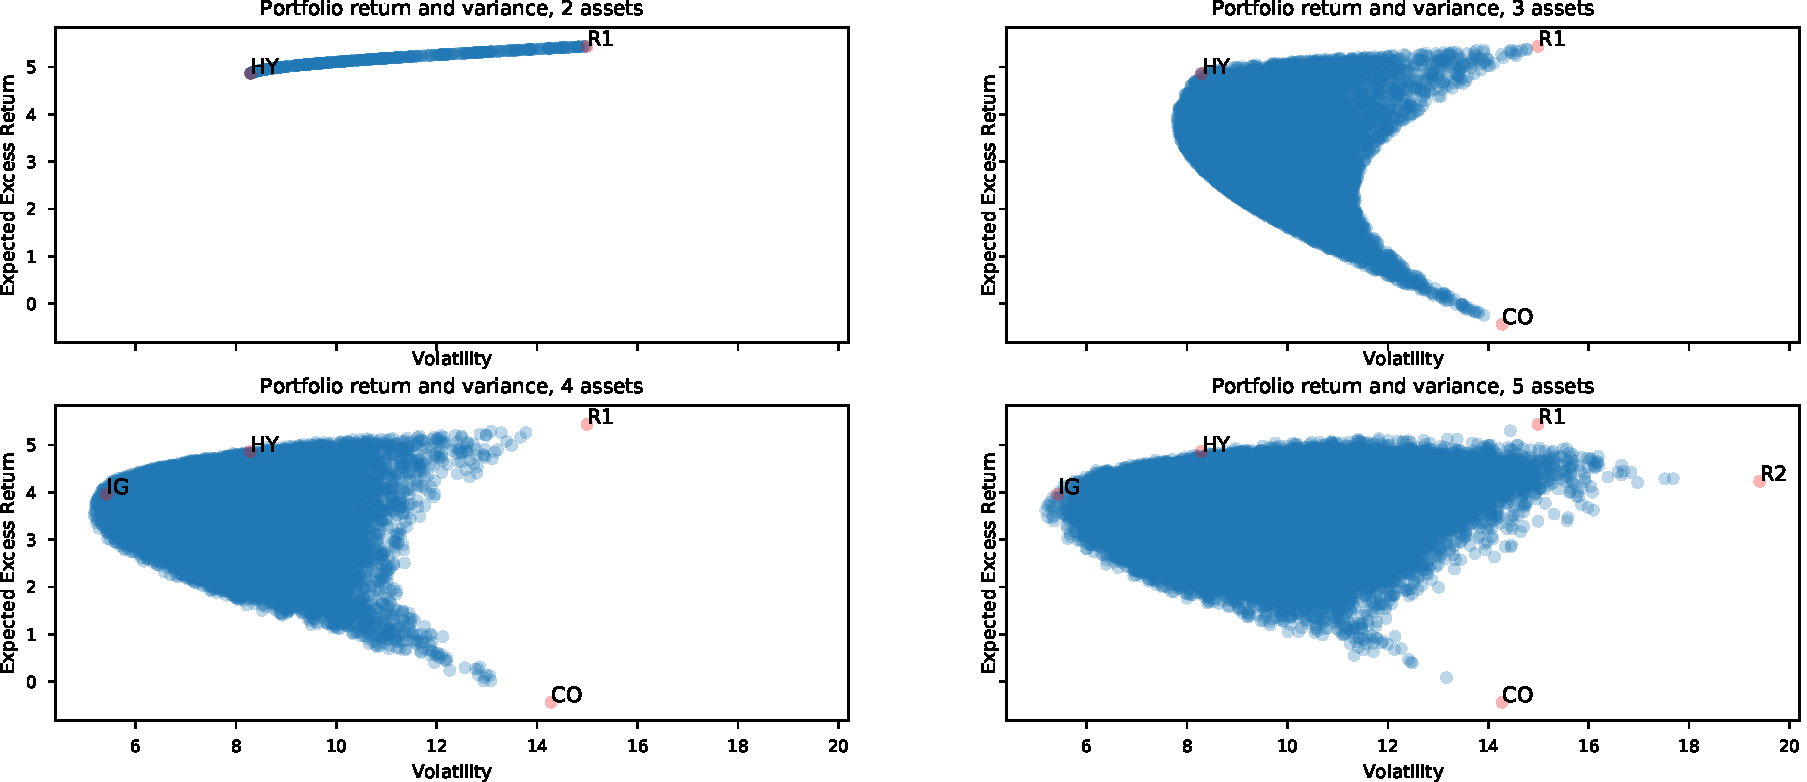
\includegraphics[scale=0.6]{images/pfAllocations.pdf}
\begingroup
\vspace{4mm}
\subcaption*{Portfolios: 2 assets: High Yield (HY) and Russell 1000 (R1000), 3 assets: HY, Commodities (C) and R1000, 4 assets: HY, C, Investment Grade bonds (IG), and R1000, 5 assets: HY, C, IG, Russell 2000 (R2000) and R1000.}
\endgroup
\end{figure}

The four panels in figure 1 show us how an expansion of the investment universe allows for a broader palette of risk-reward profiles to be satisfied. The top left panel shows us an investment universe of two assets, which provide a narrow set of portfolio choices. The top right panel expands the investment universe by one asset, effectively providing portfolios with lower variance for profiles with less appetite for risk. The bottom left panel includes a fourth asset and substantially expands the portfolio choices available to an investor, which holds true even more so for five assets.

Many of the suggested portfolios are inefficient. By definition, efficient portfolios lie on the efficient frontier. The efficient frontier is the set of portfolios which have highest expected excess return at each variance. The frontier starts at the portfolio with minimal variance, and rises to the right in a concave curve. Formally, we need to consider portfolio optimisation.

\noindent


\section{Bibliography}


\end{document}